\begin{savequote}[50mm]
---Marty, non stai pensando quadridimensionalmente!---
\qauthor{Emmett Brown} 
---Sono in ritardo! In arciritardissimo!---
\qauthor{Bianconiglio} \end{savequote}


\chapter{Logica Multimodale - Back To The Future}


\section{Logiche multimodali}

una logica multimodale è una logica che definisce oltre ai normali
operatori della logica proposizionale gli operatori:

$[i]$ con $i\in I$

$<i>\equiv\neg[i]\neg$

definita sul frame:

$F=(S,\{R_{i}\,|\, i\in I\})$ 

La semantica di una logica multimodale è la stessa della logica proposizionale
per gli operatori comuni, mentre gli operatori box hanno la seguente
semantica:

$\veraw{\mu}{\alpha}{\neci ia}\iff\veraw{\mu}{\beta}a\,\forall\beta\,:\,(\alpha,\,\beta)\in R_{i}$

Chiamiamo assioma $K_{i}$ la seguente formula:

$K_{i}$: $\neci i{(a\implies b)}\implies(\neci ia\implies\neci i{b)}$

Tutte le logiche multimodali normali devono contenere:

gli assiomi $K_{i}$ $\forall i\in I$

le regole di necessitazione:

$RN_{i}:$ $\dfrac{a}{\neci ia}$ $\forall i\in I$


\section{Futuro e Passato}

Possiamo applicare le logiche multimodali al concetto di tempo, per
farlo consideriamo il frame:

$F=(S,\,\{R_{P},\, R_{e}\})$

da cui possiamo ricavare gli operatori modali:

$[P]$ e $[F]$

ricordiamo che:

$<P>\equiv\neg[P]\neg$

$<F>\equiv\neg[F]\neg$

Perché le due relazioni rappresentino il tempo che scorre una deve
essere l'opposta dell'altra, in modo che la prima relazione rappresenti
il futuro, la seconda il passato:

$\alpha R_{P}\beta\iff\beta R_{F}\alpha$

$R_{p}=R_{f}^{-1}$

Questa proprietà si può dimostrare equivalente ai due assiomi:

$B_{PF}:$ $a\implies\necp{\posf a}$

$B_{FP}:$ $a\implies\necf{\posp a}$


\subsection{Dimostrazione}

Ip) $\veraw{\mu}{\alpha}a$ e $\forall\beta\,:\,(\alpha,\,\beta)\in R_{P}\iff(\beta,\,\alpha)\in R_{F}$

Ts) $\veraw{\mu}{\alpha}{\necp{\posf a}}$\\


Ogni mondo $\beta$ raggiunge $\alpha$ tramite $R_{F}$, e quindi:

$\veraw{\mu}{\beta}{\posf a}$

allora, usando la regola di necessitazione nel passato, possiamo scrivere:

$\veraw{\mu}{\alpha}{\necp{\posf a}}$

ma poiché per ipotesi in $\alpha$ è vera a:

$\veraw{\mu}{\alpha}{\necp{\posf a}}$

poiché abbiamo preso un $\alpha$ generico, la tesi è dimostrata.\\
Ip) $\veraw{\mu}{\alpha}{\necp{\posf a}}$

Ts) $R_{F}=R_{P}$\\


per assurdo $R_{F}\neq R_{p}$

prendiamo allora un mondo $\alpha$ in cui a $R_{P}$ non corrisponda
l'arco inverso nella relazione $R_{F}$

$V(A)=\{\alpha\}$

allora in $\beta$ poiché non si raggiunge tramite $R_{P}$ il mondo
$\alpha$ vale:

$\nonveraw{\mu}{\beta}{\posf A}$

ma poiché $\beta$ è raggiungibile da $\alpha$ tramite $R_{P}$ abbiamo:

$\nonveraw{\mu}{\alpha}{\necp{\posf A}}$

Ma allora, poiché in $\alpha$ è vera A:

$\nonveraw{\mu}{\alpha}{A\implies\necp{\posf A}}$

Assurdo! allora la tesi è dimostrata.

\begin{center} 
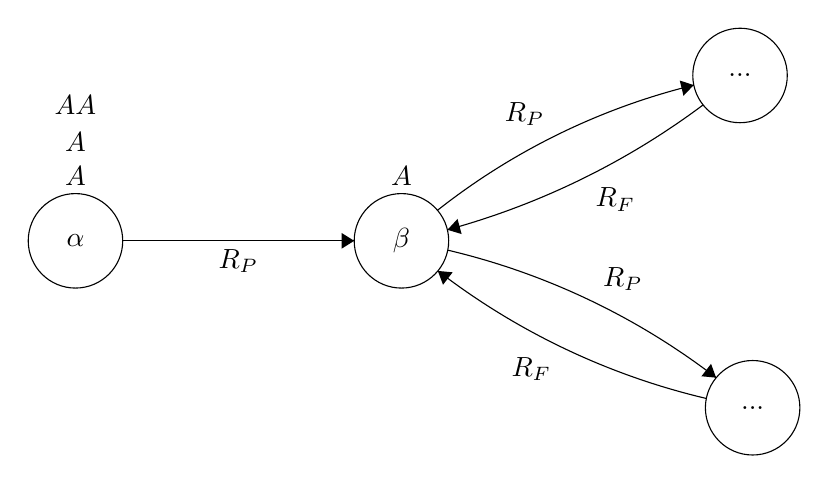
\begin{tikzpicture}[scale=0.2] 
\tikzstyle{every node}+=[inner sep=0pt] 
\draw [black] (17,-27.7) circle (3); 
\draw (17,-27.7) node {$\alpha$}; 
\draw [black] (37.7,-27.7) circle (3); 
\draw (37.7,-27.7) node {$\beta$}; 
\draw [black] (59.2,-17.2) circle (3); 
\draw (59.2,-17.2) node {$...$}; 
\draw [black] (60,-38.3) circle (3); 
\draw (60,-38.3) node {$...$}; 
\draw (17,-23.6) node {$A$}; 
\draw (37.7,-23.6) node {\sout{$\posf{A}$}}; 
\draw (17,-21.4) node {\sout{$\necp{\posf{A}}$}}; 
\draw (17,-19.1) node {\sout{$A\implies \necp{\posf{A}}$}}; 
\draw [black] (40.641,-28.292) arc (76.71074:52.44238:44.889);
\fill [black] (57.68,-36.39) -- (57.36,-35.51) -- (56.75,-36.3);
\draw (51.76,-30.92) node [above] {$R_P$}; 
\draw [black] (39.988,-25.761) arc (128.26646:103.79273:42.728);
\fill [black] (56.26,-17.81) -- (55.37,-17.52) -- (55.61,-18.49); 
\draw (45.52,-20.4) node [above] {$R_P$};
\draw [black] (20,-27.7) -- (34.7,-27.7);
\fill [black] (34.7,-27.7) -- (33.9,-27.2) -- (33.9,-28.2);
\draw (27.35,-28.2) node [below] {$R_P$}; 
\draw [black] (56.855,-19.07) arc (-53.2117:-74.72911:48.403);
\fill [black] (40.62,-27) -- (41.52,-27.27) -- (41.26,-26.31);
\draw (51.28,-24.31) node [below] {$R_F$}; 
\draw [black] (57.059,-37.71) arc (-103.2634:-127.58348:44.797); 
\fill [black] (40.01,-29.61) -- (40.34,-30.49) -- (40.95,-29.7); 
\draw (45.94,-35.08) node [below] {$R_F$}; 
\end{tikzpicture} 
\end{center}


\section{Frame Temporale}

Un frame temporale è un frame così composto:

$F=(S,\, R_{F})$

con $R_{F}=R_{p}^{-1}$ e $R_{F}$ transitiva.

In un frame temporale devono valere gli assiomi:

A1, A2, A3, $K_{P}$, $K_{F}$, $4_{P}$, $4_{F}$, $B_{FP}$, $B_{PF}$

dove gli assiomi che esprimono la transitività sono:

$4_{P}$: $\necf a\implies\necf{\necf a}$

$4_{F}$: $\necp a\implies\necp{\necp a}$

$B_{PF}:$ $a\implies\necp{\posf a}$

$B_{FP}:$ $a\implies\necf{\posp a}$\\


Una logica temporale è una logica normale multimodale nei connettivi
modali {[}F{]} e {[}P{]}

che contiene gli schemi $B_{FP}$ $B\mbox{\ensuremath{_{PF}}}$$4_{P}$
$4_{F}$.

Si dice logica lineare temporale ogni logica normale che contiene
la minima

logica normale temporale $Kt$

$Kt$ si assiomatizza con $A1,\ A2,\ A3,\ MP,\ K_{P},\ K_{F},\ B_{PF},\ B_{FP},\ 4_{P},\ 4_{F},\ RN_{P},\ RN_{F}$


\section{Correttezza, completezza e decidibilità nelle logiche multimodali}

Possiamo seguire lo stesso schema di dimostrazioni usato nella logica
unimodale per dimostrare la correttezza, completezza e decidibilità
delle logiche multimodali. Bisogna tuttavia ridefinire alcuni dettagli,
ossia il teorema di raggiungibilità e la $\Gamma$-Filtrazione


\subsection{Teorema di Raggiungibilità}

$(\alpha,\,\beta)\in R^{\Lambda}$

è equivalente a:

$\{a\,|\,\necf a\in\alpha\}\subseteq\beta$

oppure:

$\{\posf{b\,|\, b\in\beta\}\subseteq\alpha}$


\subsection{$\Gamma$-Filtrazione}

Bisogna, nel caso delle logiche multimodali, ridefinire il concetto
di relazione filtrata R'.

R' infatti dovrà ora soddisfare le tre seguenti proprietà:

F1) $(\alpha,\,\beta)\in R\implies([\alpha],\,[\beta])\in R'$

F2) $([\alpha],\,[\beta])\in R'\implies(\forall\necf b\in\Gamma\,\veraw{\mu}{\alpha}{\necf b}\implies\veraw{\mu}{\beta}b)$

F3) $([\alpha],\,[\beta])\in R'\implies(\forall\necp b\in\Gamma\,\veraw{\mu}{\beta}{\necp b}\implies\veraw{\mu}{\alpha}b)$


\section{Distinzione tra ($\mathbb{Q}$ ,<) e ($\mathbb{R}$ ,<)}

Nella logica unimodale non siamo in grado di distinguere i frame ($\mathbb{Q}$
,<) e ($\mathbb{R}$ ,<), entrambi sono espressi dalla logica K4DLX

Per convenzione poniamo:

$\boa\equiv\necp a\wedge a\wedge\necf a$

L'assioma che esprime la continuità della relazione è il seguente:

Cont: $\boxx{(\necp a\implies\posf{\necp{a)}}\implies(\necp a\implies\necf{a)}}$

Si dimostra che:

$\nonvera{(\mathbb{Q},<)}{Cont}$

$\vera{(\mathbb{R},<)}{Cont}$\\
\\
Ip) $V(A)=\{q\in\mathbb{Q}\,|\, q<\sqrt{2}\}$

Ts) $\nonvera{(\mathbb{Q},<)}{Cont}$\\


Preso $\alpha<\sqrt{2}$, varranno:

$\veraw{\mu}{\alpha}{\necp A}$

$\nonveraw{\mu}{\alpha}{\necf A}$

e quindi possiamo scrivere $\forall\alpha<\sqrt{2}$

$\nonveraw{\mu}{\alpha}{\necp A\implies\necf A}$

Tuttavia l'antecedente di Cont è vero, infatti $\forall\alpha<\sqrt{2}$:

$\veraw{\mu}{\alpha}{\posf{\necp A}}$ 

e quindi l'antecedente di Cont è vero

mentre $\forall\alpha>\sqrt{2}$ vale:

$\nonveraw{\mu}{\alpha}{\necp A}$

e quindi l'antecedente di Cont è ancora vero.

Poiché l'antecedente di Cont è sempre vero, mentre la conseguenza
no, allora:

$\nonvera{(\mathbb{Q},<)}{Cont}$

e la tesi è dimostrata.\\


  \definecolor{cc60000}{RGB}{198,0,0} \definecolor{c800000}{RGB}{128,0,0}
\begin{tikzpicture}[y=0.80pt,x=0.80pt,yscale=-1, 
inner sep=0pt, outer sep=0pt] \begin{scope}[shift={(0,-752.36216)}] 
 \path[shift={(0,752.36216)},draw=black,line join=miter,line 
cap=butt,line     width=0.800pt] (30.0000,55.0000) -- (578.6159,55.0000);
  \path[draw=cc60000,fill=c800000,line join=miter,line cap=butt,line    
width=1.176pt] (318.0000,789.0651) .. controls (317.7036,818.9733)
and     (318.0000,817.6504) .. (318.0000,817.6504);  
\path[shift={(0,752.36216)},fill=black] (344.70734,136.11012) node[above right]  
  (text3993) {};  
\path[fill=black] (305.92676,776.86609) 
node[above right] (text4078) {$\sqrt{2}$}; 

\path[shift={(0,752.36216)},fill=black] 
(489.36133,76.863548) node[above right]     (text4105) {};  
\path[draw=black,line join=miter,line cap=butt,line width=0.710pt]  
  (254.0000,817.9182) -- (254.0000,788.8061);   \path[fill=black]

(235.91389,777.67352) node[above right] (text4228) {$\alpha$};  

\path[cm={{0.09011,0.0,0.0,0.12041,(552.7687,781.39932)}},draw=black,fill=black]   
 (354.7100,211.5149) -- (302.2148,240.5337) -- (250.8362,271.4865) -- 
   (251.9528,211.5149) -- (250.8362,151.5433) -- (302.2148,182.4960) -- cycle;
\end{scope}
\end{tikzpicture} 

Ip) $\delta=\max\limits _{\eta\in\mathbb{R}}(\veraw{\mu}{\eta}{A\,\eta<\delta)}$

Ts) $\vera{(\mathbb{R},<)}{Cont}$\\


$\forall\alpha<\delta$ possiamo scrivere:

$\veraw{\mu}{\alpha}{\necp A}$

$\nonveraw{\mu}{\alpha}{\necf A}$

Tuttavia l'antecedente di Cont è falso, infatti:

$\veraw{\mu}{\delta}{\necp A}$

ma poiché non può esistere nessun mondo $\xi>\delta$ in cui sia vera
A, essendo $\delta$ massimo, avremo che:

$\nonveraw{\mu}{\delta}{\posf{\necp A}}$

e quindi non potrà che essere che:

$\veraw{\mu}{\delta}{\necp a\implies\posf{\necp a}}$

Poiché $\delta$ è raggiungibile da a avremo che:

$\veraw{\mu}{\alpha}{\boxx{(\necp a\implies\posf{\necp a})}}$

allora avremo che in $\alpha$ l'antecedente di Cont è falso solo
quando è falso il conseguente, e quindi il teorema è dimostrato.\\
\begin{tikzpicture}[y=0.80pt,x=0.80pt,yscale=-1, inner sep=0pt, outer sep=0pt] 
\begin{scope}[shift={(0,-752.36216)}]  
\path[shift={(0,752.36216)},draw=black,line join=miter,line cap=butt,line   
 width=0.800pt] (30.0000,55.0000) -- (578.6159,55.0000);  
\path[shift={(0,752.36216)},fill=black] (344.70734,136.11012) node[above right]     (text3993) {};

\path[fill=black] (360.87012,839.06793) node[above right] (text4078) {$\gamma$};  

\path[shift={(0,752.36216)},fill=black] (489.36133,76.863548) node[above right]    (text4105) {}; 
\path[draw=black,line join=miter,line cap=butt,line width=0.777pt] 
(276.0850,827.9182) -- (276.0850,799.3622);  

\path[fill=black] (210.22182,794.57617) node[above right] (text4228) {$\alpha$};

  \path[cm={{0.09011,0.0,0.0,0.12041,(552.7687,781.39932)}},draw=black,fill=black]  
  (354.7100,211.5149) -- (302.2148,240.5337) -- (250.8362,271.4865) --    
(251.9528,211.5149) -- (250.8362,151.5433) -- (302.2148,182.4960) -- cycle; 
 \path[shift={(0,752.36216)},draw=black,line join=miter,line cap=butt,line 
   width=0.800pt] (230.0000,54.5911) -- (230.0000,90.0000) -- (30.0000,90.0000);  

\path[fill=black] (263.79507,789.35651) node[above right] (text4725) {[p]a};  
\path[fill=black] (262.00568,840.79724) node[above right] (text4729) {$\delta$};  

\path[shift={(0,752.36216)},draw=black,line join=miter,line cap=butt,line    
width=0.800pt] (359.6890,47.0000) -- (359.6890,75.7800); 
\end{scope}
\end{tikzpicture}

Questo significa che esiste una differente potenza espressiva tra
la logica unimodale e la logica multimodale.


\section{Logica della concorrenza}

Una logica che si presta bene a descrivere la concorrenza, cioè un
insieme di n diversi processi che agiscono in parallelo, condividendo
la memoria, in modo che ogni processo può alterare i valori di variabili
usate anche dagli altri, è la logica nota sotto il nome di LTL (linear
temporal logic) o di logica delle concorrenza.\\
Si introducono l'operatore unario$\circ$ e l'operatore binario $U$\\
La semantica di questa logica è espressa tramite il frame detto \textbf{sequenza
di stati} che è costituito da una coppia (S,$\sigma$) dove S è al
solito un insieme di stati e $\sigma$ è una funzione suriettiva da
$\omega$ ad S e enumera gli stati di S disponendoli in sequenza (con
eventuali elementi ripetuti)

La funzione di valutazione V si da in modo consueto, tranne che per
i seguenti:

$\veraw Mj{\circ}a$, se e solo se $\veraw M{j+1}a$

$\veraw Mj{\boa}$, se e solo se $\veraw Mka$ per ogni $k\geq j$,

$\veraw Mj{aUb}$, se e solo se $\veraw Mkb$ per qualche $k\geq j$
e $\veraw Mia$ per ogni i con$j\leq i<k$.\\
\\
Questa logica si può assiomatizzare con i seguenti:\\
\\
$K_{\square}:\ \boxx{(\implica a{b)\implies(\boa\implies\boxx{b)}}}$

$K_{\circ}:\ \circ(\implica a{b)\implies(\circ a\implies\circ b)}$

$Fun:\ \circ\neg a\iff\neg\circ a$

$Mix:\ \boxx{a\implies a\wedge\circ\boa}$

$Ind:\ \boxx{(a\implies\circ a)\implies(a\implies\boa)}$

$U1:\ aUb\implies\diam b$

$U2:\ aUb\iff b\vee(a\wedge\circ(aUb))$\\


Si dimostra che LTL è determinata dai frame sequenza di stati.


\subsection{Correttezza di LTL}

Gli assiomi A1, A2, A3, $K_{\circ}$, $K_{\square}$ sono validi su
tutti i frame, e quindi portano formule vere a formule vere.

L'assioma Fun vale solo se la relazione di raggiungibilità a un passo
è una funzione: infatti se non ho stati raggiungibili da uno stato,
abbiamo che non vale $\circ a$, e quindi vale $\neg\circ a$, ma
$\circ\neg a$ non può valere perché non ci sono stati raggiungibili.
Mentre se abbiamo più di uno stato raggiungibile $\circ a$ è falso
anche se solo in uno degli stati vale $\neg a$, e quindi $\circ\neg a$
non può essere vero, perché $\neg a$ è vero solo in un successore.
Ma per definizione la raggiungibilità a un passo è una funzione.

Mix implica immediatamente lo schema T e quindi la riflessività.

4: $\boa\implies\boxx{\boa}$

Per provare la presenza di 4, notiamo che se vale 

Mix, vale anche: $\boa\implies\circ\boa$ (se vale l'and vale anche
uno solo delle due parti)

Per $RN_{\square}:\boxx{(\boa\implies\circ\boa)}$

Scrivendo Ind (con $\boa$ come $a$): $\boxx{(\boxx{a\implies\circ\boxx a)\implies(\boxx{a\implies\boxx{\boa)}}}}$ 

Per MP dalle due precedenti: $\boa\implies\boxx{\boa}$

Si può inoltre dimostrare che sono validi gli assiomi:

$L1:\,\boxx{(\boa\implies b)\vee\boxx{(\boxx b\implies a)}}$ di cui
L è una banale estensione, che indica la debole connessione del frame.

$Dum:\,(\boa\implies a)\implies(\diam{\boa\implies\boa)}$ che svolge
lo stesso ruolo di Z per la relazione $\leq$sul frame $\omega$


\subsection{CTL}

In questa logica si cerca di modellizzare l'esecuzione di più programmi
lanciati in parallelo, e quindi di fatto descrive un frame in cui
ogni nodo ha al massimo n figli.

CTL usa i seguenti operatori modali:

$[\forall F]a$: In tutte le esecuzioni c'è uno stato in cui vale
a, a è inevitabile

$[\exists F]a$: a un certo punto vale a

$[\forall G]a$: a vale in tutti gli stati dell'albero

$[\exists G]a$: esiste una sequenza di stati successivi all'attuale
tale che a è vero in ogni stato di tale sequenza

$[\forall X]a$: in tutte le esecuzioni, nello stato successivo vale
a

$[\exists X]a$: c'è uno stato successivo in cui vale a

$\forall(a\mathcal{U}b)$: in tutti i rami vale $a\mathcal{U}b$

$\exists(a\mathcal{U}b)$: in almeno un ramo vale $a\mathcal{U}b$

Tuttavia sono necessari solo tre operatori, mentre tutti gli altri
si possono ricavare, quelli indispensabili sono:

$[\forall X]a$

$\forall(a\mathcal{U}b)$

$\exists(a\mathcal{U}b)$

E infatti si dimostra facilmente che:

$[\forall F]a\equiv\forall(\top\mathcal{U}a)$

$[\exists F]a\equiv\exists(\top\mathcal{U}a)$

$[\forall F]a\equiv\neg\exists(\top\mathcal{U\neg}a)$

$[\exists F]a\equiv\neg\forall(\top\mathcal{U\neg}a)$

$[\exists xX]a\equiv\neg[\forall X]\neg a$

Si può ora assiomatizzare ctl usando solo gli operatori normali nel
seguente modo:

A1, A2, A3, MP

$K_{\forall x}:\,[\forall X](a\implies b)\implies([\forall X]a\implies[\forall X]b)$

$D_{\forall x}:\,[\exists X]\top$

$\exists U:\,\exists(a\mathcal{U}b)\iff b\vee(a\wedge[\exists X]\exists(a\mathcal{U}b))$

$\forall U:\,\forall(a\mathcal{U}b)\iff b\vee(a\wedge[\forall X]\forall(a\mathcal{U}b))$

$RN_{\forall x}:\,\dfrac{a}{[\forall x]a}$

$\exists-Ind:\,\dfrac{b\vee(a\wedge[\exists x]c)\implies c}{\exists(a\mathcal{U}b)\implies c}$

$\forall-Ind:\,\dfrac{b\vee(a\wedge[\forall x]c)\implies c}{\forall(a\mathcal{U}b)\implies c}$


\section{Logica Dinamica}


\subsection{Definizione della logica dinamica}

La logica dinamica è una logica che si occupa di descrivere le proprietà
di un programma.

L'idea è di associare a ogni istruzione $\alpha$ del programma un
operatore modale $[\alpha]a$ con il significato ``dopo ogni esecuzione
di $\alpha$ a è vera''.

L'operatore duale $<\alpha>a$ significa invece ``esiste una esecuzione
di $\alpha$, dopo la quale a è vera''.

quindi vale come al solito:

$<\alpha>\equiv\neg[\alpha]\neg$

Le logiche dinamiche si definiscono sul particolare modello:

$\mu=(S,\,\{R_{\alpha}\,|\,\alpha\in Programmi\},\, V)$

Definiamo gli insiemi:

$\phi$: insieme delle formule atomiche

$\pi$: insieme dei programmi elementari

Le formule ben formate sono definite come al solito:
\begin{itemize}
\item $a\in\phi$
\item $\neg a,\,[\alpha]a,\,<\alpha>a$ con $\alpha$ programma
\item $a\wedge b,\, a\vee b,\, a\implies b,\, a\iff b$
\item null'altro è una formula ben formata.
\end{itemize}
I programmi sono definiti come:
\begin{itemize}
\item $\alpha\in\pi$
\item $\alpha;\beta$ ossia la concatenazione di due programmi
\item $\alpha\cup\beta$ ossia non-deterministicamente $\alpha$ oppure
$\beta$
\item $\alpha^{*}$ossia la ripetizione di $\alpha$
\item $a?$ ossia il test di $\alpha$
\end{itemize}
Le relazioni che descrivono il comportamento dei programmi composti
sono espressi dalle seguenti equivalenze:

$R_{\alpha;\beta}\equiv R_{\alpha}\circ\, R_{\beta}$

$R_{\alpha\cup\beta}\equiv R_{\alpha}\cup\, R_{\beta}$

$R_{\alpha^{*}}\equiv\underset{n\geq0}{\bigcup}R_{\alpha}^{n}$

$R_{a?}\equiv\{(s,\, s)\,|\,\veraw{\mu}sa\}$


\subsection{Assiomatizzazione della logica dinamica}

La logica dinamica modale può essere assiomatizzata aggiungendo agli
schemi della logica multimodale normale, ossia gli assiomi A1, A2,
A3, $K_{[\alpha]}$ i seguenti assiomi:

Comp: $[\alpha;\beta]a\iff[\alpha][\beta]a$

Union: $[\alpha\cup\beta]a\iff[\alpha]\wedge[\beta]a$ 

Mix: $[\alpha^{*}]a\iff a\wedge[\alpha][\alpha^{*}]a$

Ind: $[\alpha^{*}](a\implies[\alpha]a)\implies(a\implies[\alpha^{*}]a)$

Test: $[a?]b\iff(a\implies b)$


\subsection{Logica dinamica concorrente proposizionale}

Si può estendere la logica dinamica, normalmente utilizzata per programmi
sequenziali, ai programmi concorrenti, aggiungendo l'operatore $[\alpha\cap\beta]a$
che significa ``dopo aver eseguito parallelamente $\alpha$ e $\beta$
è vera a''.

Per farlo tuttavia, dobbiamo modificare le relazioni del modello,
per poter gestire i casi con la concorrenza, e quindi abbiamo che:

$R_{\alpha}\subseteq S\times\mathcal{P}(S)$

E' quindi necessario cambiare pure la semantica della logica:

$\veraw{\mu}S{[\alpha]a}\iff\forall T\subseteq S\,:\,(\alpha,\, T)\in R_{\alpha}\,\wedge\,\forall t\in T\,\veraw{\mu}ta$

$\veraw{\mu}S{<\alpha>a}\iff\exists T\subseteq S\,:\,(\alpha,\, T)\in R_{\alpha}\,\wedge\,\forall t\in T\,\veraw{\mu}ta$

Si nota quindi che:

$[\alpha]\not\equiv\neg<\alpha>\neg$

Allora è necessario ridefinire il prodotto tra relazioni:

$(s,\, T)\in R_{\alpha}\circ\, R_{\beta}\iff\exists U\subseteq\mathcal{P}(S)\,\wedge\,(s,\, U)\in R_{\alpha}\,\wedge\,\forall u\in U\exists T_{u}\,:\,(u,\, T_{u})\in R_{\beta}\,\wedge\, T=\underset{u\in U}{\bigcup T_{u}}$

Il prodotto di relazioni è quindi cambiato, passando dal seguente
grafo:

\begin{center} 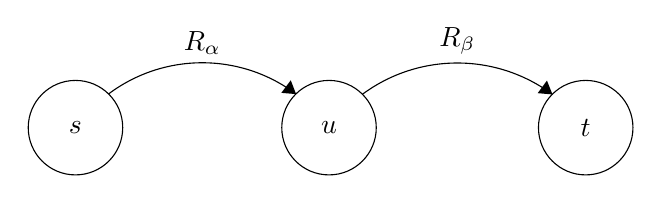
\begin{tikzpicture}[scale=0.2] \tikzstyle{every node}+=[inner sep=0pt] \draw [black] (21.4,-15.1) circle (3); \draw (21.4,-15.1) node {$s$}; \draw [black] (37.5,-15.1) circle (3); \draw (37.5,-15.1) node {$u$}; \draw [black] (53.8,-15.1) circle (3); \draw (53.8,-15.1) node {$t$}; \draw [black] (23.492,-12.966) arc (126.89872:53.10128:9.923); \fill [black] (35.41,-12.97) -- (35.07,-12.09) -- (34.47,-12.89); \draw (29.45,-10.48) node [above] {$R_\alpha$}; \draw [black] (39.613,-12.986) arc (126.52967:53.47033:10.141); \fill [black] (51.69,-12.99) -- (51.34,-12.11) -- (50.75,-12.91); \draw (45.65,-10.49) node [above] {$R_\beta$}; \end{tikzpicture} \end{center}

Al seguente grafo:

\definecolor{cffffff}{RGB}{255,255,255}
\begin{tikzpicture}[y=0.80pt,x=0.80pt,yscale=-1, inner sep=0pt, outer sep=0pt]   \path[cm={{0.58805,0.0,0.0,0.68269,(24.31388,102.98422)}},draw=black,fill=cffffff]     (156.7931,87.4161)arc(0.000:180.000:50.387171 and     44.750)arc(-180.000:0.000:50.387171 and 44.750) -- cycle;   \path[fill=black] (82.20771,167.96637) node[above right] (text3755) {s};   \path[cm={{0.74795,0.0,0.0,0.85608,(68.60394,12.42678)}},draw=black,fill=cffffff]     (265.1861,106.6421)arc(0.000:180.000:73.920640 and     42.098)arc(-180.000:0.000:73.920640 and 42.098) -- cycle;   \path[fill=black] (180.73416,65.26226) node[above right] (text3763) {U};   \path[draw=black,line join=miter,line cap=butt,line width=0.800pt]     (110.0523,145.4256) -- (164.8679,122.9266);   \path[cm={{0.71337,0.0,0.0,0.47229,(79.07095,130.99431)}},draw=black,fill=cffffff]     (265.1861,106.6421)arc(0.000:180.000:73.920640 and     42.098)arc(-180.000:0.000:73.920640 and 42.098) -- cycle;   \path[draw=black,line join=miter,line cap=butt,line width=0.800pt]     (113.3671,174.5960) -- (163.5672,177.9203);   \path[shift={(-12.0,0)},draw=black,fill=cffffff]     (236.0157,85.7587)arc(-0.038:180.038:13.922)arc(-180.038:0.038:13.922) --     cycle;   \path[cm={{0.92174,0.0,0.0,0.92174,(-3.13845,9.35718)}},draw=black,fill=cffffff]     (245.2972,119.5699)arc(-0.021:180.021:14.916721 and     12.596)arc(-180.021:0.021:14.916721 and 12.596) -- cycle;   \path[fill=black] (200,89.362183) node[above right] (text3817) {u1};   \path[fill=black] (200.91348,124.35682) node[above right] (text3817-5) {u2};   \path[fill=black] (124.37474,126.52254) node[above right] (text3842) {$R_\alpha$};   \path[fill=black] (127.6106,171.96516) node[above right] (text3846) {$R_\alpha$};   \path[cm={{0.8212,0.0,0.0,0.49268,(188.32152,21.20068)}},draw=black,fill=cffffff]     (265.1861,106.6421)arc(0.000:180.000:73.920640 and     42.098)arc(-180.000:0.000:73.920640 and 42.098) -- cycle;   \path[cm={{0.8212,0.0,0.0,0.42066,(180.68016,98.39161)}},draw=black,fill=cffffff]     (265.1861,106.6421)arc(0.000:180.000:73.920640 and     42.098)arc(-180.000:0.000:73.920640 and 42.098) -- cycle;   \path[draw=black,line join=miter,line cap=butt,line width=0.800pt]     (222.6493,122.0455) -- (286.4164,133.7944);   \path[draw=black,line join=miter,line cap=butt,line width=0.723pt]     (221.3768,77.3255) -- (285.5725,77.2936);   \path[shift={(99.17758,-11.35244)},draw=black,fill=cffffff]     (236.0157,85.7587)arc(-0.038:180.038:13.922)arc(-180.038:0.038:13.922) --     cycle;   \path[cm={{0.92174,0.0,0.0,0.92174,(102.03913,32.00475)}},draw=black,fill=cffffff]     (245.2972,119.5699)arc(-0.021:180.021:14.916721 and     12.596)arc(-180.021:0.021:14.916721 and 12.596) -- cycle;   \path[fill=black] (315.17758,78.00975) node[above right] (text3817-0) {t1};   \path[fill=black] (306.09106,147.00439) node[above right] (text3817-5-7) {t3};   \path[shift={(139.67676,-10.5883)},draw=black,fill=cffffff]     (236.0157,85.7587)arc(-0.038:180.038:13.922)arc(-180.038:0.038:13.922) --     cycle;   \path[cm={{0.92174,0.0,0.0,0.92174,(142.53831,32.76888)}},draw=black,fill=cffffff]     (245.2972,119.5699)arc(-0.021:180.021:14.916721 and     12.596)arc(-180.021:0.021:14.916721 and 12.596) -- cycle;   \path[fill=black] (353.67676,78.773872) node[above right] (text3817-6) {t2};   \path[fill=black] (346.59024,147.76852) node[above right] (text3817-5-6) {t4};   \path[fill=black] (326.2858,46.646969) node[above right] (text3942) {T1};   \path[fill=black] (324.32019,122.09327) node[above right] (text3942-3) {T2};   \path[fill=black] (248.34399,146.86179) node[above right] (text3990) {$R_\beta$};   \path[fill=black] (253.16176,74.356461) node[above right] (text3990-7) {$R_\beta$};   \path[fill=black,line join=miter,line cap=butt,line width=0.800pt] (0,0)     node[above right] (flowRoot4015) {};   \path[draw=black,line join=miter,line cap=butt,line width=0.800pt]     (401.1048,36.8263) .. controls (409.7612,32.3735) and (435.8124,31.6775) ..     (440.0757,44.4676) .. controls (444.4570,57.6116) and (438.5475,69.8092) ..     (438.5475,84.2027) .. controls (438.5475,89.4537) and (452.1943,92.7158) ..     (448.4812,96.4288) .. controls (445.2189,99.6911) and (435.7460,104.0714) ..     (438.5475,112.4757) .. controls (442.6528,124.7916) and (450.2611,160.1129) ..     (443.8964,172.8424) .. controls (440.9921,178.6510) and (417.3816,176.6631) ..     (411.0386,176.6631);   \path[fill=black] (462.52805,101.66471) node[above right] (text4174) {T};
\end{tikzpicture}\\


Bisogna cambiare anche la Relazione di iterazione nel seguente modo:

$R_{\alpha^{*}}\equiv\underset{n\geq0}{\bigcup}R_{\alpha}^{n}$ con
$R_{\alpha}^{0}=\{(s,\,\{s\})\,|\, s\in S\}$ e $R_{\alpha}^{n}=R_{\alpha}\circ\, R_{\alpha}^{n-1}$ 

Inoltre si introduce la relazione di combinazione, ossia quella che
traduce il parallelismo (l'operatore intersezione):

$(s,\, T)\in R_{\alpha}\otimes R_{\beta}\iff T=U\cup V\,\wedge\,(s,U)\in R_{\alpha}\,\wedge\,(s,V)\in R_{\beta}$

Tutto il resto è definito allo stesso modo di prima, a meno di stare
attenti agli insiemi di stati, anziché agli stati.
